\section{Organización del proyecto}
\label{organiz}

Para incentivar el trabajo en paralelo en proyecto, se han creado diferentes grupos de trabajo identificados por las tareas que conllevan:

\begin{figure}[h]
	\centering 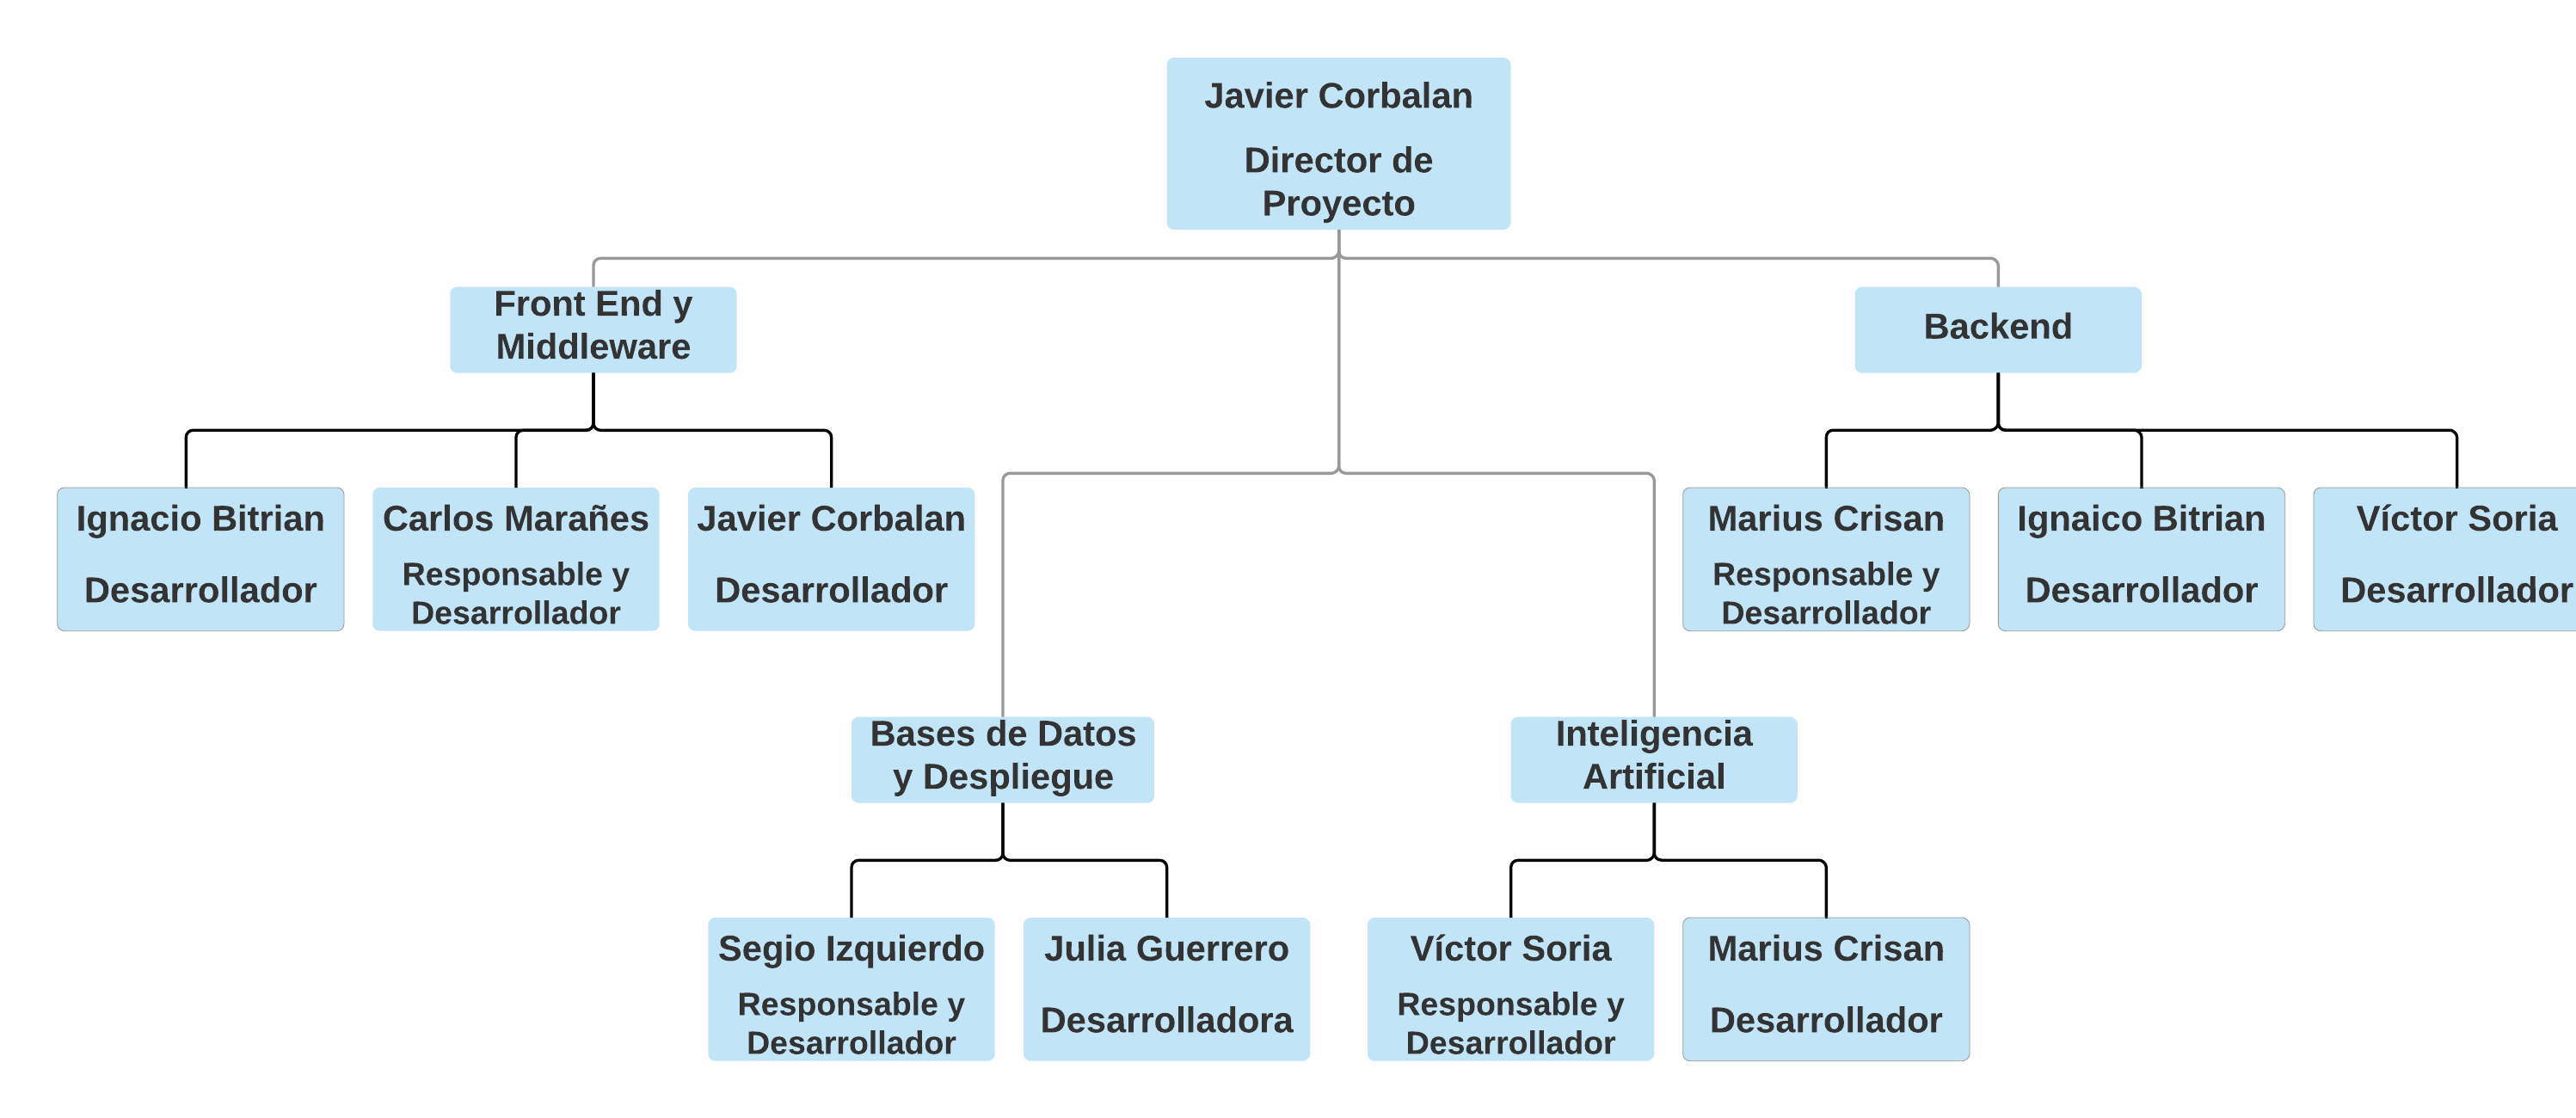
\includegraphics[scale=0.6]{figuras/organigrama.png}
\end{figure}


\begin{enumerate}
\item Desarrollo del Frontend y Middleware: Incluye el desarrollo de la interfaz y las vistas de la aplicación, además de la gestión de la comunicación entre los jugadores y servidor durante el desarrollo la partida.
	\begin{itemize}
    \item Carlos Marañés \textbf{(responsable)}.
		\item Javier Corbalán.
    	\item Ignacio Bitrián.
	\end{itemize}
\newpage
\item Despliegue e implementación de la base de datos: Incluye el análisis y diseño de la base de datos, gestión de los datos de carácter personal de los usuarios acorde con la LOPD\footnote{\href{http://www.agpd.es/portalwebAGPD/canaldocumentacion/informes_juridicos/reglamento_lopd/index-ides-idphp.php}{Ley Orgánica de Protección de Datos}} , despliegue de la aplicación y mantenimiento.
	\begin{itemize}
    	\item Sergio Izquierdo \textbf{(responsable)}.
        \item Julia Guerrero.
    \end{itemize}
\item Desarrollo de la inteligencia artificial: Incluye el análisis del juego, diseño e implementación de un agente de inteligencia artificial.
	\begin{itemize}
    	\item Victor Soria \textbf{(responsable)}.
        \item Marius Crisan.
    \end{itemize}
\item Desarrollo del Backend: Implementación de los servicios web, tratamiento de peticiónes, generación de páginas dinámicas y la lógica del juego.
	\begin{itemize}
   		\item Marius Crisan \textbf{(responsable)}.
    	\item Ignacio Bitrian.
        \item Víctor Soria.
    \end{itemize}
\end{enumerate}

El rol de director del proyecto corre a cargo de Javier Corbalán. La elección del director se ha llevado a cabo através de una votación de mayoría simple.
